\chapter{Introduzione ai Sistemi Operativi}
\newpage

\section{Cos'è un sistema operativo? }

\textbf{Definizione:} Un sistema operativo è un programma che controlla l'esecuzione di
programmi applicativi e agisce come interfaccia tra le applicazioni e l'hardware del calcolatore.


\begin{itemize}
    \item Efficenza: Un S.O. cerca di utilizzare in modo efficiente le risorse del calcolatore
    \item Semplicità: Un sistema operativo dovrebbe semplificare l'utilizzazione dell'hardware di
    un calcolatore
\end{itemize}

\paragraph{S.O come gestione di risorse:}
Gestendo le risorse di un calcolatore, un S.O. controlla il
funzionamento del calcolatore stesso. Ma questo controllo è esercitato in modo "particolare".
Normalmente, il meccanismo di controllo è esterno al sistema controllato.

\textit{Esempio: termostato e impianto di riscaldamento}
\newline
In un elaboratore, il S.O. è un programma, simile all'oggetto del controllo, ovvero le applicazioni controllate. Il S.O. deve lasciare il controllo alle applicazioni e affidarsi al
processore per riottenere il controllo.

\begin{figure} [h]
    \centering
    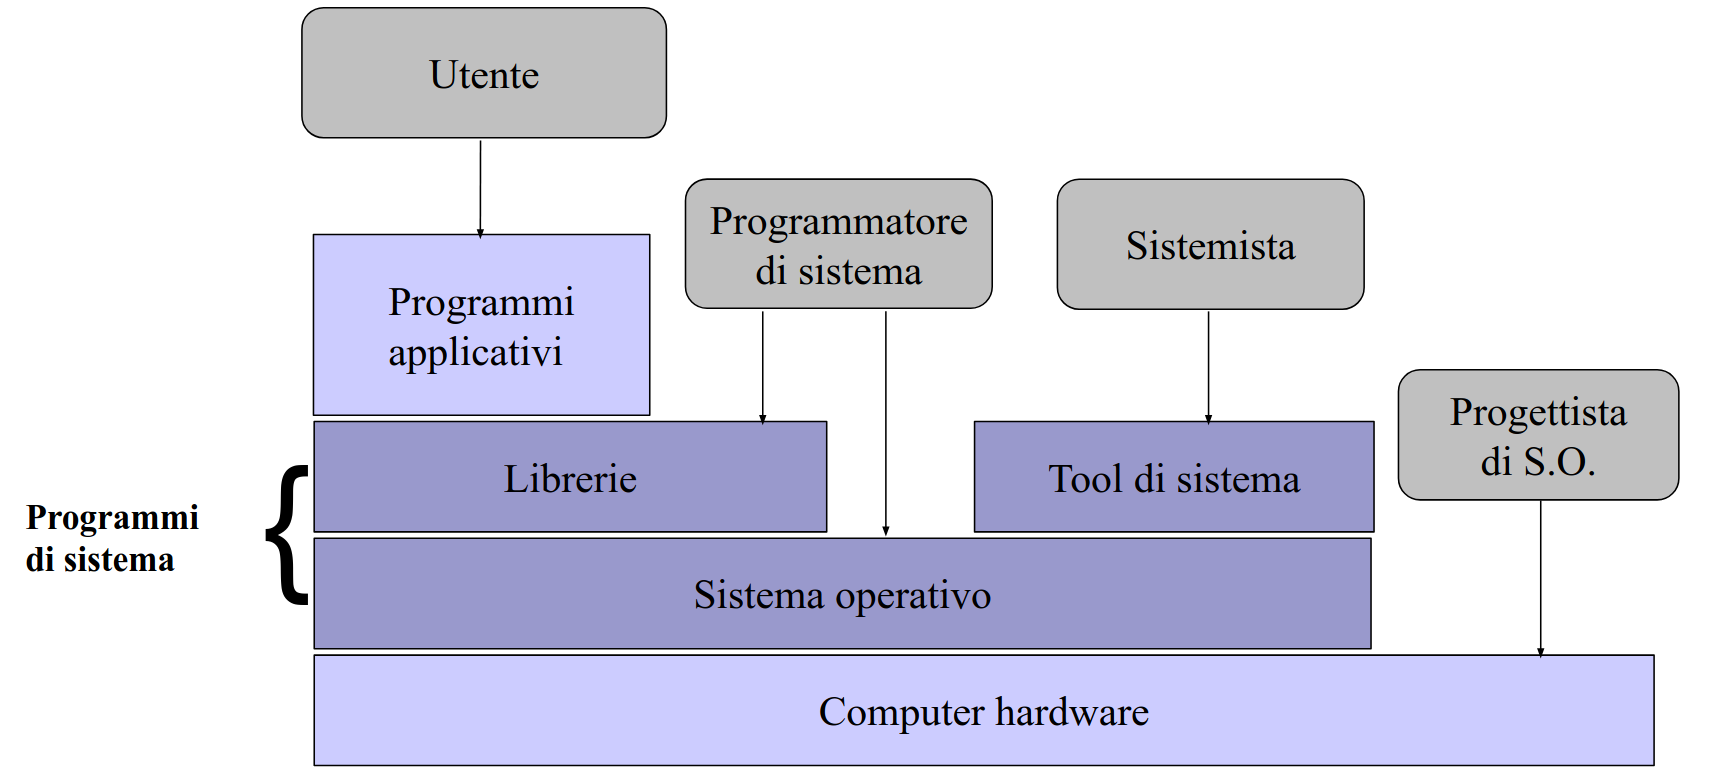
\includegraphics[width=0.7\linewidth]{Images/Screenshot 2024-12-15 at 18-55-32 so-01-intro-os.pptx - so-01-intro-os.pdf.png}
    \caption{Un S.O nasconde ai programmatori i dettagli dell'hardware e fornisce ai programmatori una API conveniente e facile da usare, agisce come intermediario tra programmatore e hardware.}
     \label{fig:Figura1}
\end{figure}

\textbf{S.O come macchina estesa}

\begin{multicols}{2}
   \begin{lstlisting}
//Esempio senza S.O.
li $t0, 0xDEFF12 // init
sw $t0, 0xB000.0040
li $t0, 0xFFDF // motor
sw $t0, 0xB000.0044
li $t0, 0xFFBB
sw $t0, 0xBOOO.0048
...
\end{lstlisting}
    \columnbreak
    \begin{lstlisting}[language=]
//Esempio con S.O.
fd = open("/etc/rpc");
read(fd, buffer, size);
\end{lstlisting}
\end{multicols}

\begin{center}
    \small\textit{NB: Questo è esempio serve a dare un'idea,
la realtà è molto più complessa \dots}
\end{center}

\paragraph{Servizi estesi offerti da un S.O.}
\begin{itemize}
\item[-] esecuzione di programmi
\item[-] accesso semplificato ai dispositivi di I/O
\item[-] accesso controllato a dispositivi, file system, etc.
\item[-] accesso al sistema
\item[-] rilevazione e risposta agli errori
\item[-] accounting
\end{itemize}

\subsection{Tipi di sistemi}

\subsubsection{Sistemi Paralleli}
\textbf{Definizione:} Un sistema parallelo è un singolo elaboratore che possiede più unità di elaborazione. Si dicono anche sistemi tightly coupled.
Alcune risorse contenute nell'elaboratore possono essere condivise.
\textit{Esempio: Memoria}
La comunicazione avviene tramite memoria condivisa o canali di
comunicazione dedicati.

\paragraph{Vantaggi dei sistemi paralleli}
    \begin{itemize}
        \item incremento delle prestazioni
        \item incremento dell’affidabilità (graceful degradation)
    \end{itemize}

\paragraph{Tassonomia basata sulla struttura}
 \begin{itemize}
\item \textbf{SIMD} - Single Instruction, Multiple Data: Le CPU              eseguono all'unisono lo stesso programma su dati diversi
\item \textbf{MIMD} - Multiple Instruction, Multiple Data: Le CPU            eseguono programmi differenti su dati differenti
\end{itemize}

\paragraph{Tassonomia basata sulla dimensione}

A seconda del numero (e della potenza) dei processori si suddividono in:
\begin{itemize}
\item sistemi a basso parallelismo
pochi processori in genere molto potenti
\item sistemi massicciamente paralleli
gran numero di processori, che possono avere anche potenza non elevata
\end{itemize}

\subsubsection{Sistemi Distribuiti}
\textbf{Definizione:} Sono sistemi composti da più elaboratori indipendenti (con proprie risorse e
proprio sistema operativo)
Si dicono anche sistemi loosely coupled.
Ogni processore possiede la propria memoria locale e sono collegati tramite linee di comunicazione (rete, linee
telefoniche, linee wireless, etc)

\paragraph{Vantaggi dei sistemi distribuiti}
    \begin{itemize}
    \item Condivisione di risorse
    \item Suddivisione di carico, incremento delle prestazioni
    \item Affidabilità
    \item Possibilità di comunicare
\end{itemize}

I Sistemi operativi di rete forniscono condivisione di file, la possibilità di comunicare e ogni computer opera indipendentemente dagli altri.

I Sistemi operativi distribuiti offrono minore autonomia tra i computer e danno l'impressione che un singolo sistema operativo stia controllando la rete

\subsubsection{Sistemi real-time}
\textbf{Definizione:} Sono i sistemi per i quali la correttezza del risultato non dipende solamente dal suo valore ma anche dall'istante nel quale il risultato viene prodotto

I sistemi real-time si dividono in:
\begin{itemize}
    \item hard real-time: se il mancato rispetto dei vincoli temporali può avere effetti catastrofici. \textit{e.g. controllo assetto velivoli, controllo centrali nucleari.}
    \item soft real-time: se si hanno solamente disagi o disservizi \textit{e.g. programmi interattivi}
\end{itemize}

\newpage
\section{Concetti base di architetture
degli elaboratori}

\begin{figure} [h]
    \centering
    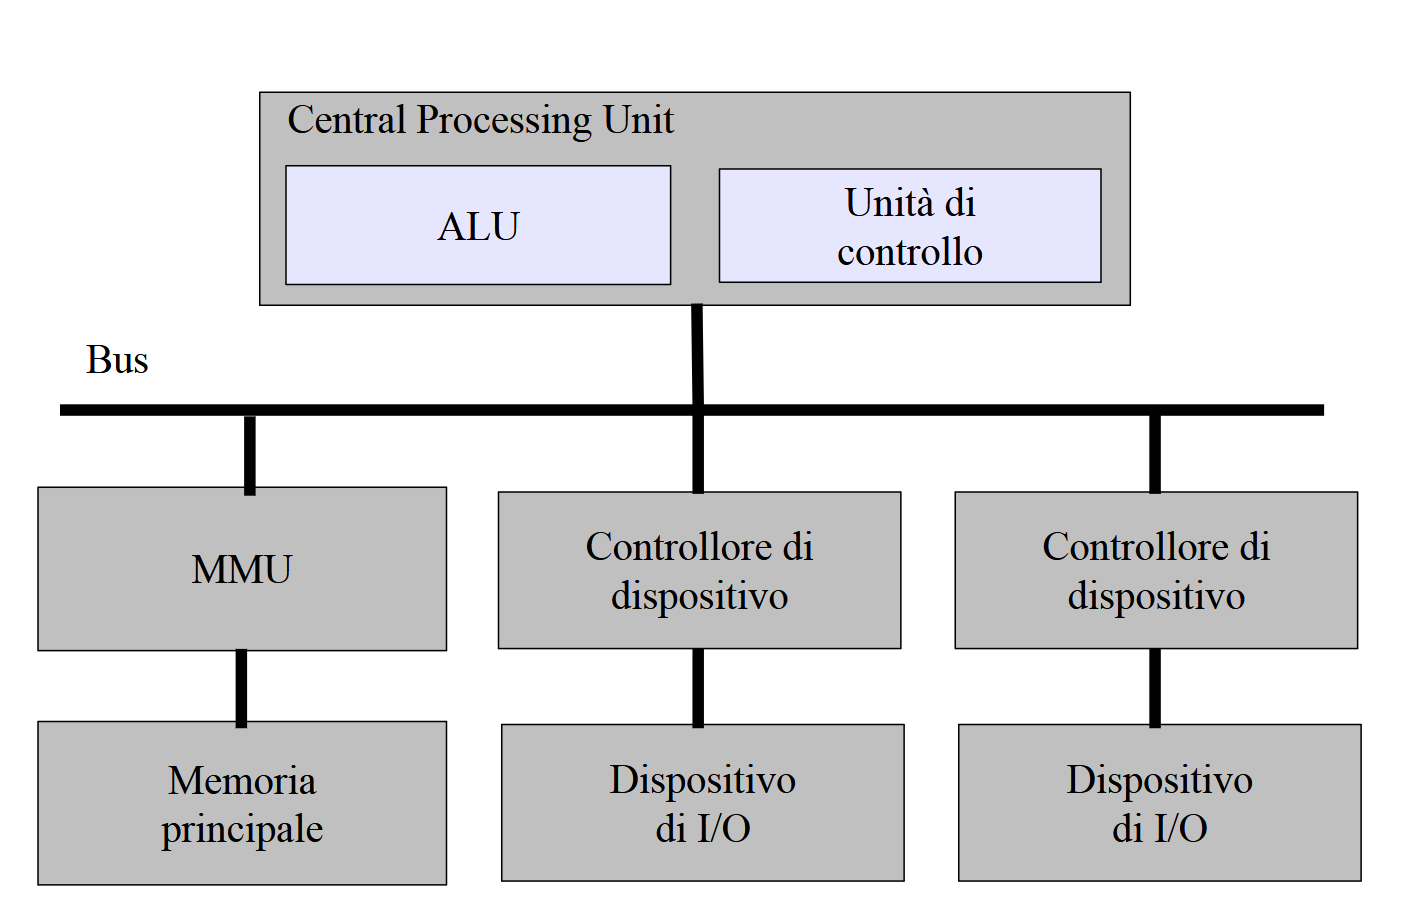
\includegraphics[width=0.5\linewidth]{Images/Screenshot 2024-12-16 125618.png}
    \caption{Architettura di Von Neumann}
    \label{fig:von-neumann1}
\end{figure}

\subsection{Interrupt}
\textbf{Definizione:} Un meccanismo che permette l'interruzione del normale ciclo di esecuzione della CPU.

Le caratteristiche: introdotti per aumentare l'efficienza di un sistema di calcolo, permettono ad un S.O. di "intervenire" durante l'esecuzione di un processo utente, allo scopo di gestire efficacemente le risorse del calcolatore.
\textit{Esempio:} processore, memoria, dispositivi di I/O

Gli interrupt possono essere sia hardware che software (detti \underline{trap})
e possono essere mascherati (ritardati) se la CPU sta svolgendo compiti non interrompibili.

\subsubsection{Interrupt vs Trap}

\begin{itemize}
    \item[-] Interrupt Hardware: eventi hardware asincroni, non causati dal processo in esecuzione

\textit{Esempi: dispositivi di I/O
(per notifica di eventi quali il completamento di una operazione di I/O), clock (scadenza del quanto di tempo)}
\item[-] Interrupt Software (Trap): Causato dal programma

\textit{Esempi: eventi eccezionali come divisione per 0 o problemi di indirizzamento, richiesta di servizi di sistema.(system call)}
\end{itemize}

\subsubsection{Gestione Interrupt - Panoramica}
Cosa succede in seguito ad un interrupt.
\newline

\textbf{Dal lato software:}
\begin{enumerate}
    \item Un segnale "interrupt request" viene spedito al processore.
    \item Il processore sospende le operazioni del processo corrente e salta ad un particolare indirizzo di memoria contenente la routine di gestione dell'interrupt (\underline{interrupt handler}).
\end{enumerate}




\textbf{Dal lato hardware}
\begin{enumerate}
    \item L'interrupt handler gestisce nel modo opportuno l'interrupt e ritorna il controllo al processo interrotto (o a un altro processo, nel caso di scheduling).
    \item Il processore riprende l'esecuzione del processo interrotto come se nulla fosse successo
\end{enumerate}
\newpage
\begin{figure} [h]
    \centering
    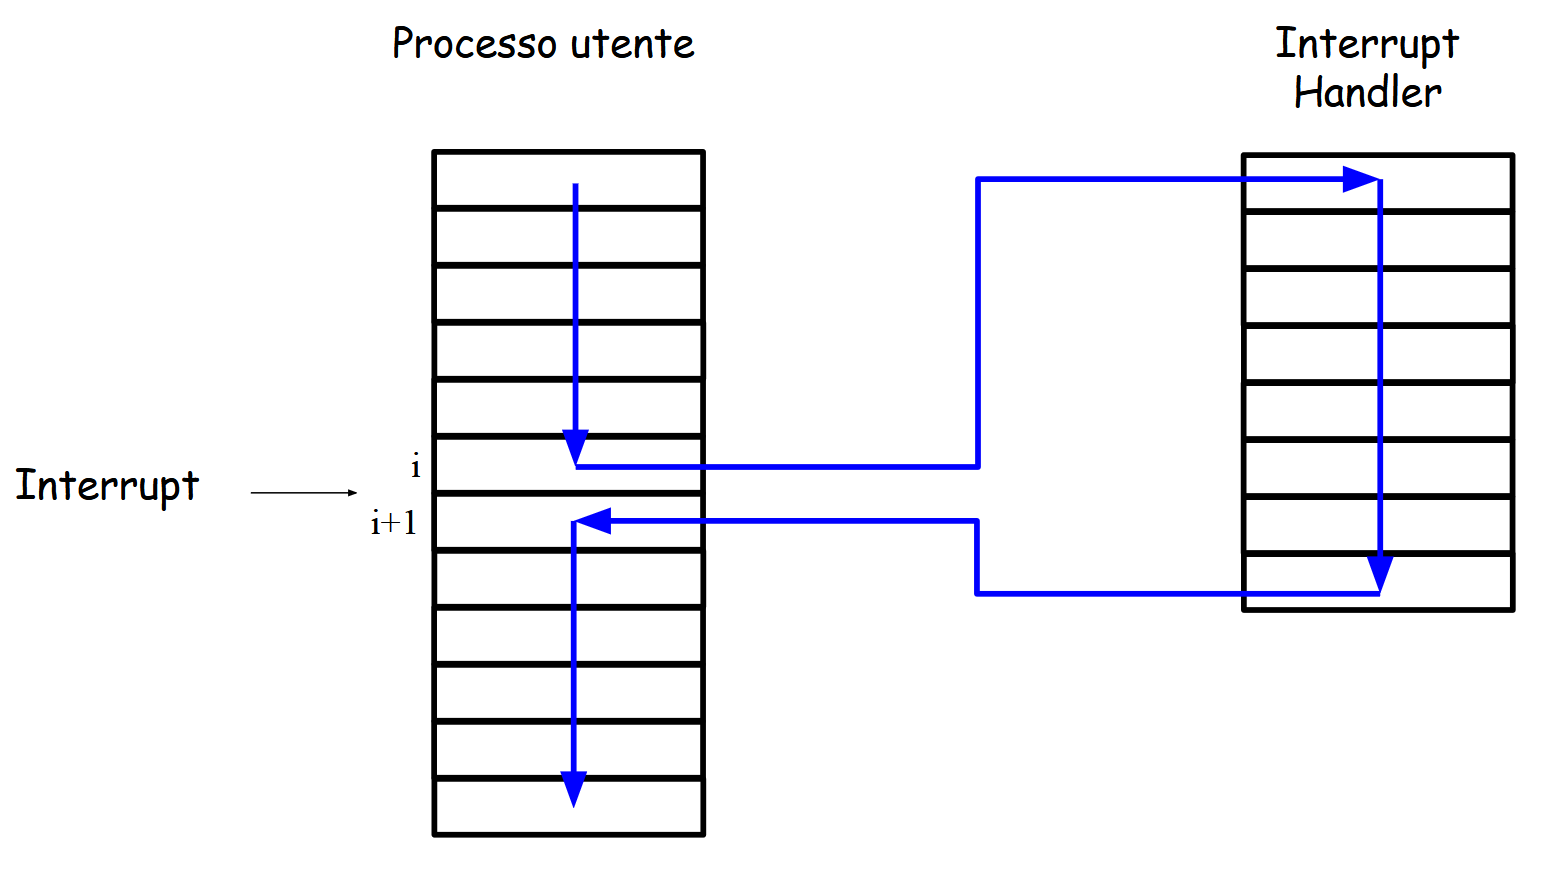
\includegraphics[width=0.7\linewidth]{Images/Screenshot 2024-12-16 132614.png}
    \label{fig:interrupt1}
\end{figure}

\subsubsection{Gestione Interrupt - Dettagli}

\begin{enumerate}
    \item Un segnale di interrupt request viene spedito alla CPU.
    \item La CPU finisce l'esecuzione dell'istruzione corrente.
    \item La CPU verifica la presenza di un segnale di interrupt, e
in caso affermativo spedisce un segnale di conferma al device
che ha generato l'interrupt.

\begin{figure} [h]
    \centering
    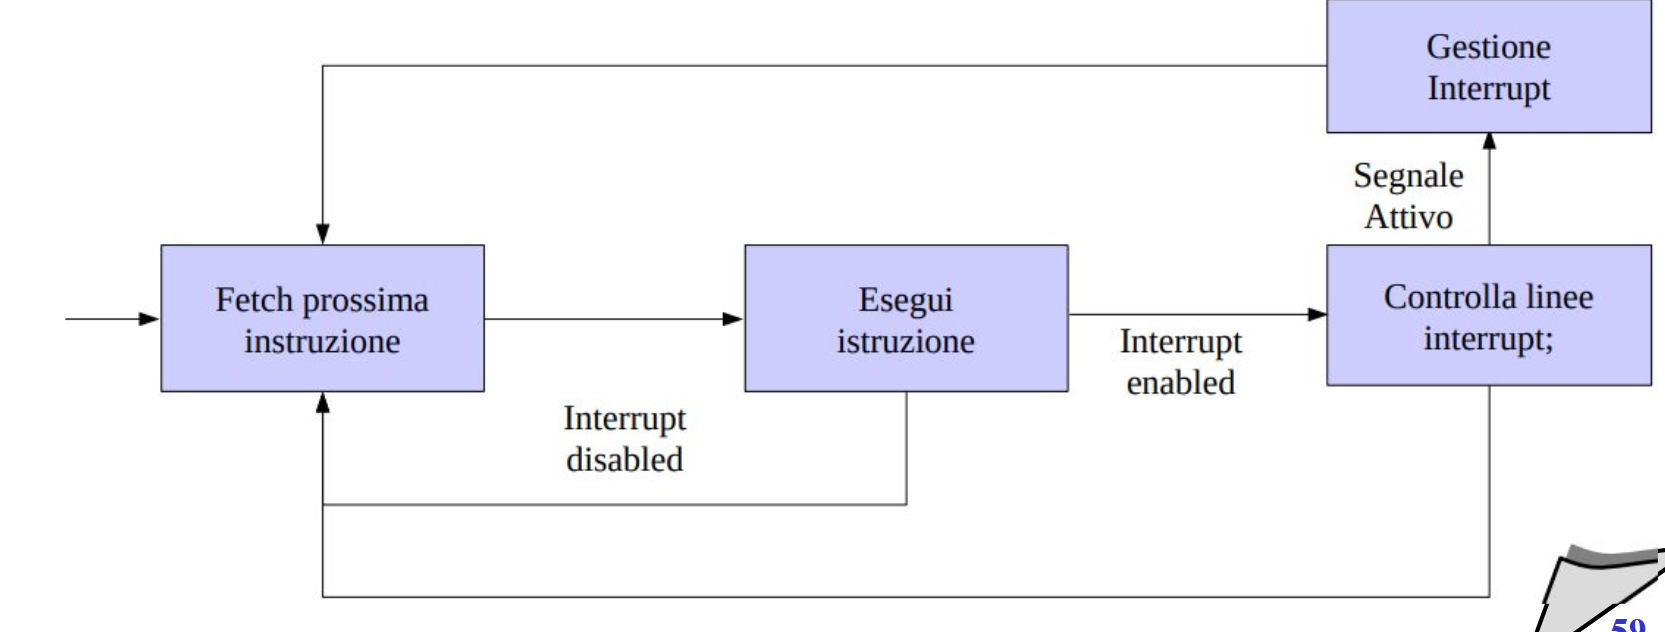
\includegraphics[width=0.7\linewidth]{Images/Screenshot 2024-12-16 132946.png}
    \label{fig:enter-label}
\end{figure}

\item  Preparazione al trasferimento di controllo dal programma all'interrupt handler
\item Selezione dell'interrupt handler appropriato a seconda dell'architettura, vi può essere un singolo interrupt handler,
uno per ogni tipo di interrupt o uno per dispositivo. La selezione avviene tramite l'interrupt vector.
\item Caricamento del PC con l'indirizzo iniziale dell'interrupt handler assegnato.

\small \textit{Nota: tutte le operazioni compiute fino a qui sono operazioni hardware, la modifica del PC corrisponde ad un salto al codice dell'interrupt handler.
A questo punto: il ciclo fetch-execute viene ripreso il controllo è passato in mano all'interrupt handler.}
\item Salvataggio dello stato del processore: salvataggio delle informazioni critiche non salvate automaticamente
dai meccanismi hardware di gestione interrupt.
\item Gestione dell'interrupt: 
lettura delle informazioni di controllo proveniente dal dispositivo. Eventualmente, spedizione di ulteriori informazioni al dispositivo stesso.
\item Ripristino dello stato del processore
l'operazione inversa della numero 7.
\item Ritorno del controllo al processo in esecuzione
(o ad un altro processo, se necessario).


\end{enumerate}


\subsubsection{Interrupt Multipli}
 La discussione precedente prevedeva la presenza di un singolo
interrupt.
Esiste la possibilità che avvengano interrupt multipli ad esempio, originati da dispositivi diversi, un interrupt può avvenire durante la gestione di un interrupt precedente.
\newline
Esistono due approcci possibili: disabilitazione degli interrupt e interrupt annidati.
\newline

\textbf{Disabilitazione Interrupt:}
durante l'esecuzione di un interrupt handler ulteriori segnali di interrupt vengono ignorati, i segnali corrispondenti restano pendenti. Gli interrupt vengono riabilitati prima di riattivare il processo interrotto e il processore verifica quindi se vi sono ulteriori interrupt, in caso attiva l'interrupt handler corrispondente.
\newline

\underline{Vantaggi e svantaggi:}
\newline
Approccio semplice, interrupt gestiti in modo sequenziale,  non tiene conto di gestioni "time-critical".

\begin{figure} [h]
    \centering
    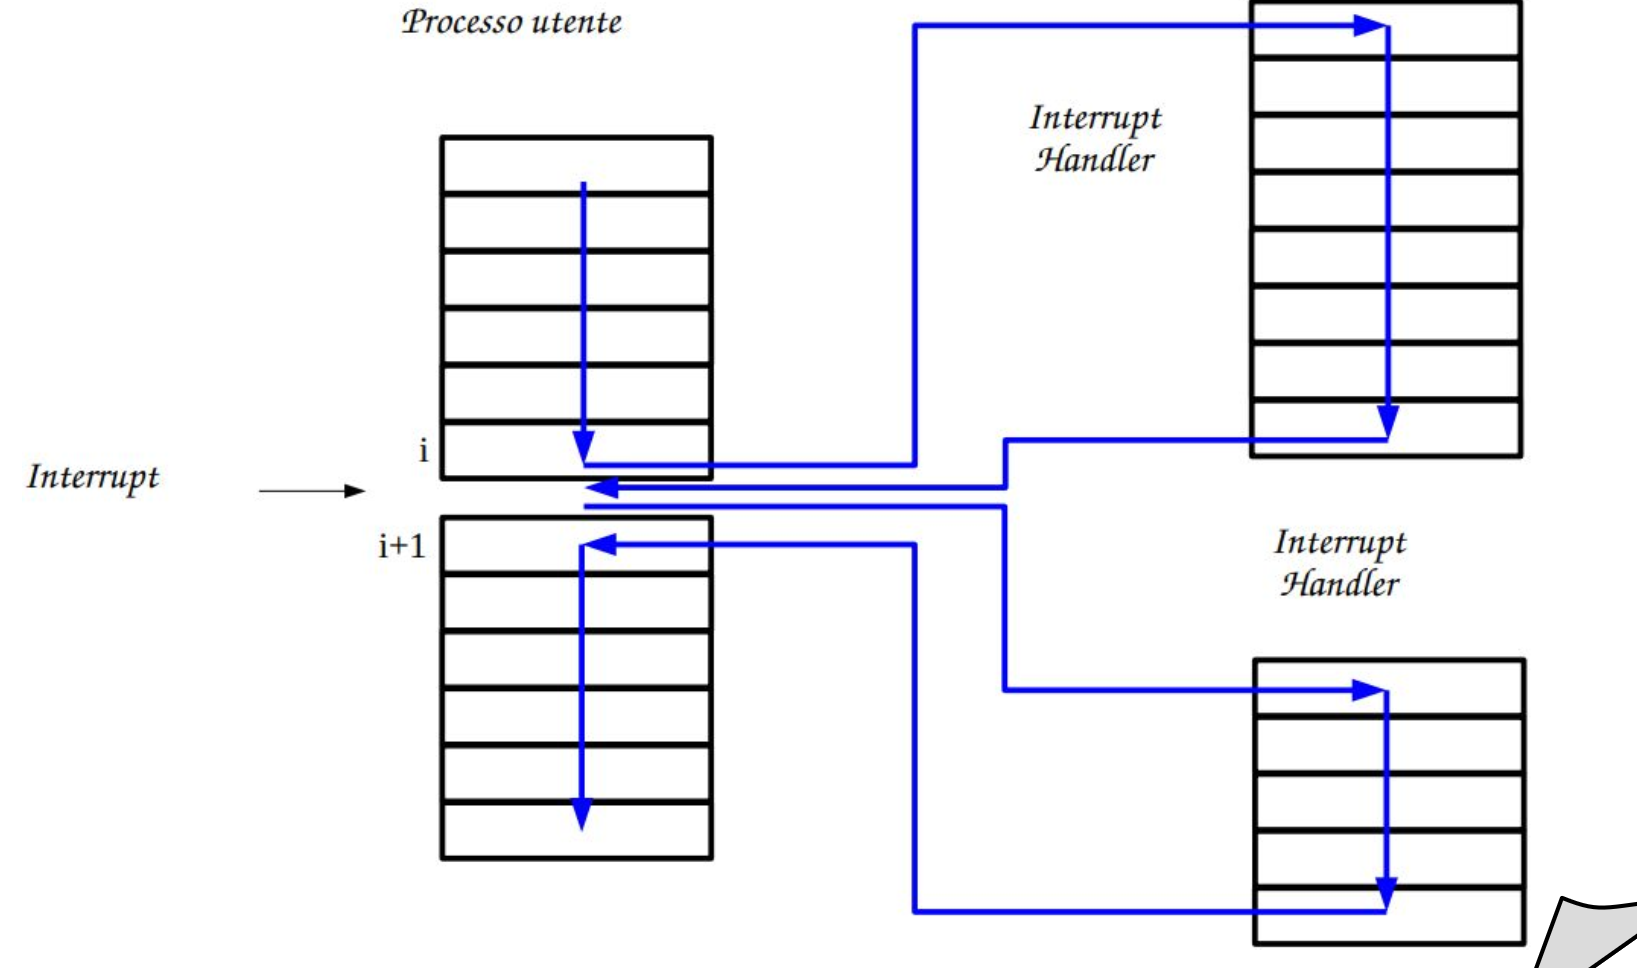
\includegraphics[width=0.7\linewidth]{Images/Screenshot 2024-12-16 140040.png}
    \label{fig:enter-label}
\end{figure}

\textbf{Interrupt Annidati:}
E' possibile definire priorità diverse per gli interrupt. Un interrupt di priorità inferiore può essere interrotto da un interrupt di priorità superiore. Necessario prevedere un meccanismo di salvataggio e ripristino dell'esecuzione adeguato.
\newline

\underline{Vantaggi e svantaggi:}
\newline
dispositivi veloci possono essere serviti prima (es. schede di rete), approccio più complesso.

\begin{figure} [h]
    \centering
    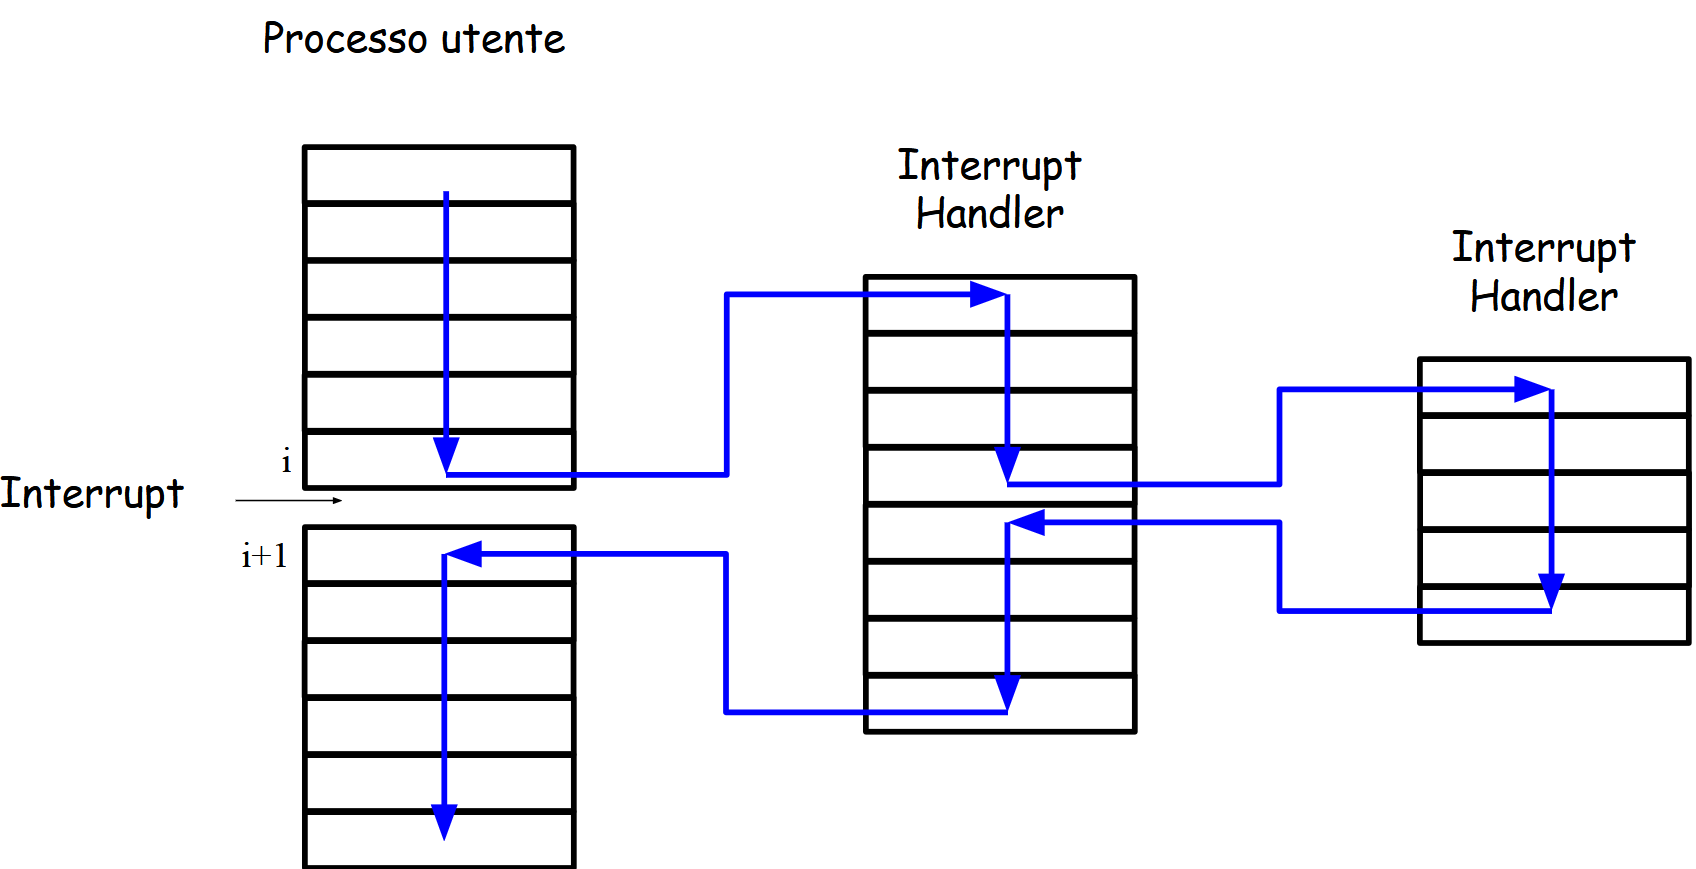
\includegraphics[width=0.7\linewidth]{Images/Screenshot 2024-12-16 140334.png}

    \label{fig:enter-label}
\end{figure}

\subsection{Comunicazione fra processore e dispositivi di I/O}
Il controllore governa il dialogo con il dispositivo fisico, il controllo della politica di accesso al dispositivo è a carico del dispositivo stesso

\textit{Esempio:
il controller di un disco accetta una richiesta per volta, 
l'accodamento delle richieste in attesa è a carico del S.O.}
\newline

Esistono 3 modalità di controllo;
\begin{enumerate}
    \item Programmed I/O
    \item Interrupt-Driven I/O
    \item Direct Memory Access (DMA)
\end{enumerate}

\subsubsection{Programmed I/O (obsoleto)}
\textbf{Operazione di input:}
\newline
La CPU carica (tramite il bus) i parametri della richiesta di input in appositi registri del controller (registri comando).

Il dispositivo esegue la richiesta, il risultato dell'operazione viene memorizzato in un apposito buffer locale sul controller. Il completamento dell'operazione viene segnalato attraverso appositi registri di status.

Il S.O. attende (busy waiting) che il comando sia completato
verificando periodicamente il contenuto del registro di stato.

Infine, la CPU copia i dati dal buffer locale del controller alla memoria.

\subsubsection{Interrupt-Driven I/O}
\textbf{Operazione di input:}
\newline
La CPU carica (tramite il bus) i parametri della richiesta di input in appositi registri del controller (registri comando).

Il S.O. sospende l'esecuzione del processo che ha eseguito
l'operazione di input ed esegue un altro processo.

Il dispositivo esegue la richiesta, il risultato dell'operazione viene memorizzato in un apposito buffer locale sul controller, il completamento dell'operazione viene segnalato attraverso interrupt.

Al ricevimento dell'interrupt, la CPU copia i dati dal buffer locale del controller alla memoria.

\subsubsection{Programmed I/O vs Interrupt-Driven I/O}
Nel caso di operazioni di output il procedimento è similare:
\begin{itemize}
    \item i dati vengono copiati dalla memoria ai buffer locali.
    \item questa operazione viene eseguita prima di caricare i parametri della richiesta nei registri di comando dei dispositivi.
\end{itemize}

\textbf{Svantaggi dei due approcci:}
\begin{itemize}
    \item il processore spreca parte del suo tempo nella gestione del trasferimento dei dati.
    \item la velocità di trasferimento è limitata dalla velocità con cui il processore riesce a gestire il servizio.
\end{itemize}

\subsubsection{Direct Memory Access (DMA)}

Il S.O. attiva l'operazione di I/O specificando l'indirizzo in memoria di destinazione (Input) o di provenienza (Output) dei dati.

L'interrupt specifica solamente la conclusione dell'operazione di I/O.
\newline

\textbf{Vantaggi e svantaggi:}
\begin{itemize}
    \item c'è contesa nell'accesso al bus device driver più semplici.
    \item efficace perché la CPU non accede al bus ad ogni ciclo di clock.
\end{itemize}

\subsection{Memoria}
\subsubsection{Memory Mapped I/O}
Un dispositivo è completamente indirizzabile tramite bus.
I registri di dispositivo vengono mappati su un insieme di indirizzi di memoria, una scrittura su questi indirizzi causa il trasferimento di dati verso il dispositivo.
\textit{Esempio: video grafico nei PC.}
\newline

\textbf{Vantaggi e svantaggi:}
\begin{itemize}
    \item gestione molto semplice e lineare.
    \item necessità di tecniche di polling.
\end{itemize}
\subsubsection{Dischi}
Sono dispositivi che consentono la memorizzazione non volatile dei dati permettono accesso diretto. Per individuare un dato sul disco (dal punto di vista fisico) occorre indirizzarlo in termini di cilindro, testina, settore.

Le operazioni gestite dal controller sono: READ (head, sector), WRITE(head, sector), SEEK(cylinder).

L'operazione di seek:
Corrisponde allo spostamento fisico del pettine di testine da
un cilindro ad un altro ed è normalmente la più costosa

L'operazione di read e write:
prevedono l'attesa che il disco ruoti fino a quando il settore richiesto raggiunge la testina.

\subsubsection{Gerarchia di memoria}
Trade off: Quantità, velocità, costo.
\newline
Limitazioni:
\begin{itemize}
    \item tempo di accesso più veloce, costo maggiore.
    \item maggiore capacità, costo minore (per bit).
    \item maggiore capacità, tempo di accesso maggiore.
\end{itemize}
Soluzione: utilizzare una gerarchia di memoria.
\begin{figure}[h]
    \centering
    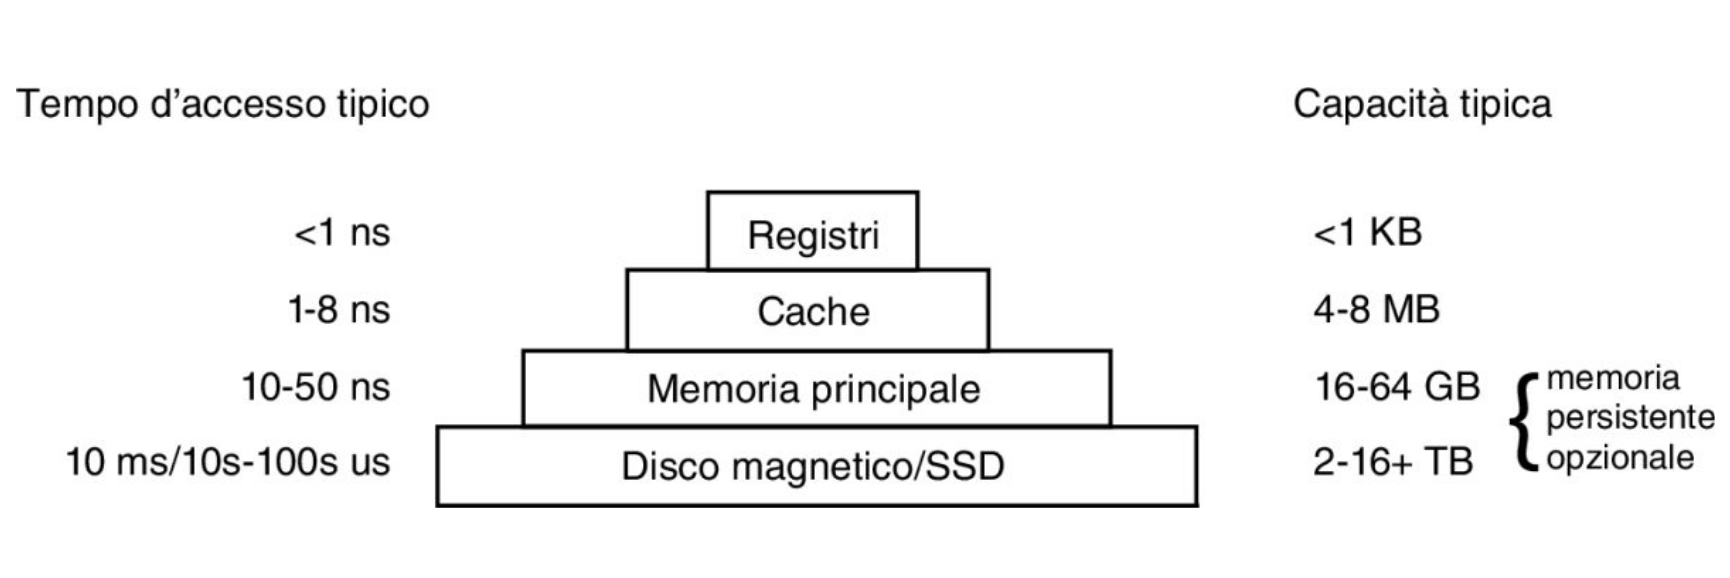
\includegraphics[width=0.7\linewidth]{Images/Screenshot 2024-12-17 at 19-02-22 so-01-intro-os.pptx - so-01-intro-os.pdf.png}
    \label{fig:enter-label}
\end{figure}

\subsubsection{Cache}
Un meccanismo di caching consiste nel memorizzare parzialmente i dati di una memoria in una
seconda più costosa ma più efficiente. Se il numero di occorrenze in cui il dato viene trovato nella cache
(memoria veloce) è statisticamente rilevante rispetto al numero totale degli accessi, la cache fornisce un notevole aumento di prestazione.

E' un concetto che si applica a diversi livelli: cache della memoria principale (DRAM), cache di disco in memoria, cache di file system remoti tramite file system locali.

I meccanismi di caching si distinguono in due modi:
\begin{itemize}
    \item \textbf{Hardware} ad esempio cache CPU; politiche non modificabili dal S.O.
    \item \textbf{Software} ad esempio cache disco; politiche sotto controllo del S.O.
\end{itemize}
I problemi da considerare nel S.O. sono molteplici. Come l' algoritmo di replacement, data la dimensione limitata della cache bisogna scegliere un algoritmo che garantisca il maggior numero di accessi in cache. Oppure la coerenza, gli stessi dati possono apparire a diversi livelli della struttura di memoria.

\subsection{Protezione Hardware}
I sistemi multiprogrammati e multiutente richiedono la presenza di meccanismi di protezione. Bisogna evitare che processi concorrenti generino interferenze non
previste, ma soprattutto bisogna evitare che processi utente interferiscano con il sistema operativo.

Quindi i meccanismi di protezione possono essere realizzati totalmente in software, oppure abbiamo bisogno di meccanismi hardware dedicati?
\newpage
\subsubsection{Modo utente / Modo kernel}
\paragraph{Modalità kernel / supervisore / privilegiata:}
I processi in questa modalità hanno accesso a tutte le istruzioni, incluse quelle privilegiate, che permettono di gestire totalmente il sistema.
\paragraph{Modalità utente:} 
I processi non hanno accesso alle istruzioni privilegiate.
\newline
Il mode bit è un bit utilizzato nei processori per distinguere tra due modalità operative: modalità kernel e modalità utente.

\paragraph{Come funziona?}
Alla partenza, il processore è in modalità kernel.
Viene caricato il sistema operativo (bootstrap) e si inizia ad eseguirlo, quando passa il controllo ad un processo utente, il S.O. cambia il valore del mode bit e il processore passa in modalità utente.
Tutte le volte che avviene un interrupt, l'hardware passa da modalità utente a modalità kernel.

\subsubsection{Protezione I/O}
Le istruzioni di I/O devono essere considerate privilegiate, il S.O. dovrà fornire agli utenti primitive e servizi per accedere all'I/O. Tutte le richieste di I/O passano attraverso codice del S.O. e possono essere controllate preventivamente.
\textit{Esempio: accesso al dispositivo di memoria secondaria che ospita un file system. Vogliamo evitare che un qualunque processo possa accedere al dispositivo modificando (o corrompendo) il file system stesso.}

\subsubsection{Protezione Memoria}
La protezione non è completa se non proteggiamo anche la
memoria, altrimenti, i processi utente potrebbero: modificare il codice o i dati di altri processi utenti, modificare il codice o i dati del sistema operativo, modificare l'interrupt vector, inserendo i propri gestori degli interrupt.

La protezione avviene tramite la \textbf{Memory Management Unit(MMU).}

\paragraph{Registro base + registro limite:} ogni indirizzo generato dal processore viene confrontato con due registri,
detti base e limite. Se non incluso in questo range, l'indirizzo non è valido e genera un'eccezione.
\paragraph{Traduzione indirizzi logici in indirizzi fisici:} ogni indirizzo generato dal processore corrisponde ad un indirizzo logico, l'indirizzo logico viene trasformato in un indirizzo fisico a tempo di esecuzione dal meccanismo di MMU.
Un indirizzo viene protetto se non può mai essere generato
dal meccanismo di traduzione.

\begin{figure} [h]
    \centering
    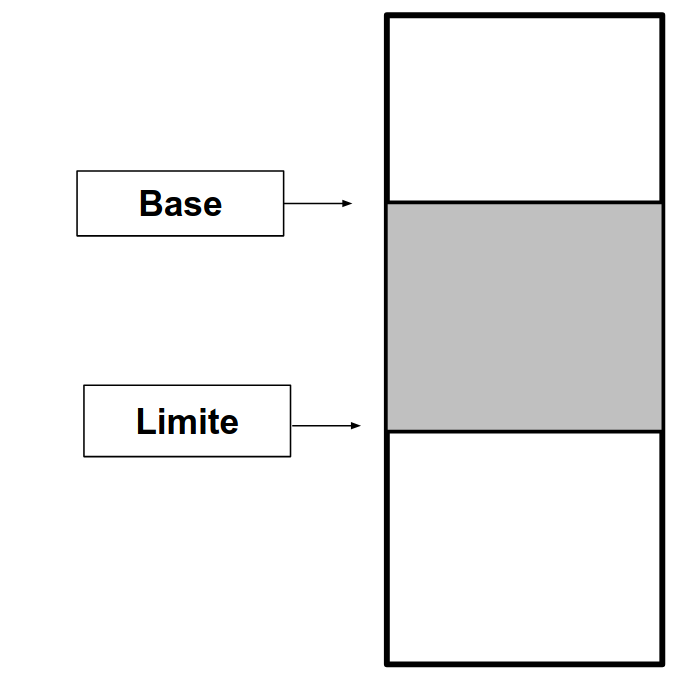
\includegraphics[width=0.3\linewidth]{Images/Screenshot 2024-12-17 at 19-31-43 so-01-intro-os.pptx - so-01-intro-os.pdf.png}
    \label{fig:enter-label}
\end{figure}

\newpage
\section{Struttura dei sistemi operativi
(panoramica)}

\subsection{Architettura dei sistemi operativi}
L'architettura di un sistema operativo descrive quali sono le varie componenti del S.O. e come queste sono
collegate fra loro. I vari sistemi operativi sono molto diversi l'uno dall'altro nella loro architettura, la progettazione di essa è un problema fondamentale.

L'architettura di un S.O. da diversi punti di vista:
servizi forniti (visione utente), interfaccia di sistema (visione programmatore), componenti del sistema (visione progettista S.O.)

\subsubsection{Le componenti di un S.O:}
\begin{enumerate}
    \item Gestione dei processi
    \item Gestione della memoria principale
    \item Gestione della memoria secondaria
    \item Gestione file system
    \item Gestione dei dispositivi di I/O
    \item Protezione
    \item Networking
    \item Interprete dei comandi
\end{enumerate}

\paragraph{Gestione dei processi}
Un processo è un programma in esecuzione che utilizza le risorse fornite dal computer per assolvere i propri compiti.

Il sistema operativo è responsabile delle seguenti attività riguardanti la gestione dei processi: creazione e terminazione dei processi, sospensione e riattivazione dei processi, gestione dei deadlock, comunicazione tra processi
e sincronizzazione tra processi.

\paragraph{Gestione della memoria principale}
La memoria principale è un "array" di byte indirizzabili singolarmente. Consideriamolo un deposito di dati facilmente accessibile e condiviso tra la CPU ed i dispositivi di I/O.

Il sistema operativo è responsabile delle seguenti attività
riguardanti la gestione della memoria principale: tenere traccia di quali parti della memoria sono usate e da chi, decidere quali processi caricare quando diventa disponibile spazio in memoria e allocare e deallocare lo spazio di memoria quando necessario.

\paragraph{Gestione della memoria secondaria}
Poiché la memoria principale è volatile e troppo piccola per contenere tutti i dati e tutti i programmi in modo permanente, un computer è dotato di memoria secondaria.
In generale, la memoria secondaria è data da hard disk, dischi ottici, nastri, etc.

Il sistema operativo è responsabile delle seguenti attività
riguardanti la gestione della memoria secondaria: Allocazione dello spazio inutilizzato, Gestione dello spazio di memorizzazione e ordinamento efficiente delle richieste (disk scheduling).

\paragraph{Gestione file system}
Un file è l'astrazione informatica di un archivio di dati.
Il concetto di file è indipendente dal media sul quale viene
memorizzato (che ha caratteristiche proprie e propria organizzazione fisica). Un file system è composto da un insieme di file. 

Il sistema operativo è responsabile delle seguenti attività
riguardanti la gestione del file system: creazione e cancellazione di file, creazione e cancellazione di directory, manipolazione di file e directory e codifica del file system sulla memoria secondaria.

\paragraph{Gestione dei dispositivi di I/O}
La gestione dell’I/O richiede: un’interfaccia comune per la gestione dei device driver, un insieme di driver per dispositivi hardware specifici e un sistema di gestione di buffer per il caching delle informazioni.

\paragraph{Protezione}
Il termine protezione si riferisce al meccanismo per controllare gli accessi di programmi, processi o utenti alle risorse del sistema e degli utenti.

Il meccanismo di protezione software deve: distinguere tra uso autorizzato o non autorizzato, specificare i controlli che devono essere imposti e fornire un meccanismo di attuazione della protezione.

\paragraph{Networking}
Consente di far comunicare due o più elaboratori, condividere risorse, utilizzando servizi come: protocolli di comunicazione a basso livello, TCP/IP, UDP, comunicazione ad alto livello, file system distribuiti (NFS, SMB) e print spooler.

\paragraph{Interprete dei comandi}
Interfaccia utente - S.O. .
Può attivare un programma, terminare un programma, interagire con le componenti del sistema operativo (file system).
Può essere: grafica (a finestre, icone, etc.), testuale (linea di comando).
Può cambiare il "linguaggio" utilizzato, ma il concetto è lo stesso, d'altronde vi sono differenze di espressività
\newline
\small\textit{N.B L'interprete dei comandi usa i servizi dei gestori di processi, I/O, memoria principale e secondaria}

\subsection{System Call}

\subsubsection{Cos'è la system call}
\paragraph{Problema:} poiché le istruzioni di I/O sono privilegiate, possono essere eseguite unicamente dal S.O. . Com'è possibile per i processi utenti eseguire operazioni di I/O?
\paragraph{Soluzione:} i processi utenti devono fare richieste esplicite di I/O al S.O. . Questo introduce il meccanismo delle system call, ovvero trap generate da istruzioni specifiche.
\newline

Ogni volta che un processo ha bisogno di un servizio del S.O.
richiama una system call. Sono in genere disponibili come istruzioni a livello assembler, esistono librerie che permettono di invocare le system call da diversi linguaggi \textit{(ad es. librerie C)}.
Vengono normalmente realizzate tramite interrupt software.
Le system call sono specifiche dei vari sistemi operativi.
\newline

Esempi di istruzioni privilegiate eseguibili in Kernel Mode:
\small\begin{itemize}
    \item Gestione della memoria
    \item Gestione della memoria virtuale (allocazione, etc.)
    \item Controllo dell'hardware (I/O, controller di interrupt)
    \item Gestione della CPU
    \item Istruzioni di halt e riavvio
    \item Gestione del clock di sistema
    \item Operazioni sulla cache
    \item Gestione dell'alimentazione
    \item Operazioni crittografiche hardware
    \item Gestione delle eccezioni e degli interrupt
    \item Accesso a registri di controllo speciali
    \item \dots
\end{itemize}





\subsubsection{Gestione dei file}

\begin{lstlisting} 
    pid = fork() //crea un processo figlio identico al padre
\end{lstlisting}

\begin{lstlisting} 
    pid = waitpid(pid, &statloc, options) //aspetta la terminazione di un processo figlio
\end{lstlisting}

\begin{lstlisting} 
    s = execve(name, argv, environment) //esegue un programma
\end{lstlisting}

\begin{lstlisting} 
    exit(status) //termina l'esecuzione del processo corrente
\end{lstlisting}

\begin{lstlisting} 
//Un programma che genera un processo figlio:
int main(void) {
    int pid;
    pid = fork();
    if (pid > 0) {
        printf('Padre\n');
    } else if (pid == 0) {
        printf('Figlio\n');
    } else {
        printf('Errore!\n');
    }
}
\end{lstlisting}

\subsubsection{Gestione del file system e delle directory}
\begin{lstlisting}
  s = mkdir(name, mode) //Crea una nuova directory  
\end{lstlisting}

\begin{lstlisting}
  s = rmdir(name) //Cancella una directory 
\end{lstlisting}

\begin{lstlisting}
  s = link(name1, name2) //Crea un nuovo link ad un file esistente
\end{lstlisting}

\begin{lstlisting}
 s = unlink(name) //Cancella un file  
\end{lstlisting}

\begin{lstlisting}
   s = mount(special, name, flag) //Monta una partizione nel file system
\end{lstlisting}

\begin{lstlisting}
   s = umount(special) //Smonta una partizione
\end{lstlisting}

\subsubsection{Varie}

\begin{lstlisting}
   s = chdir(dirname) //Cambia la directory corrente
\end{lstlisting}

\begin{lstlisting}
   s = chmod(name, mode) //Cambi i bit di protezione di un file
\end{lstlisting}

\begin{lstlisting}
   s = kill(pid, signal) //Spedisce un segnale ad un processo
\end{lstlisting}

\begin{lstlisting}
   seconds = time(&seconds) //Restituisce il tempo di sistema
\end{lstlisting}
\newpage
\subsection{File Speciali (UNIX)}
I file speciali sono pensati per far sì che i dispositivi di I/O siano visti come file.
\paragraph{I file speciali a blocchi:}
usati per modellare dispositivi costituiti da un insieme di blocchi indirizzabili in modo casuale (SSD, dischi). Aprendo un file speciale a blocchi e leggendo il blocco 4, un programma può accedere direttamente al quarto blocco, senza considerare la struttura del file system
\paragraph{I file speciali a caratteri:}
usati per modellare stampanti, tastiere, mouse, etc. che accettano una sequenza di caratteri in output, contenuti nella directory /dev.

\subsubsection{Pipe}
Una pipe è una specie di pseudo-file che può essere usato per
connettere due processi.
\begin{figure}[h]
    \centering
    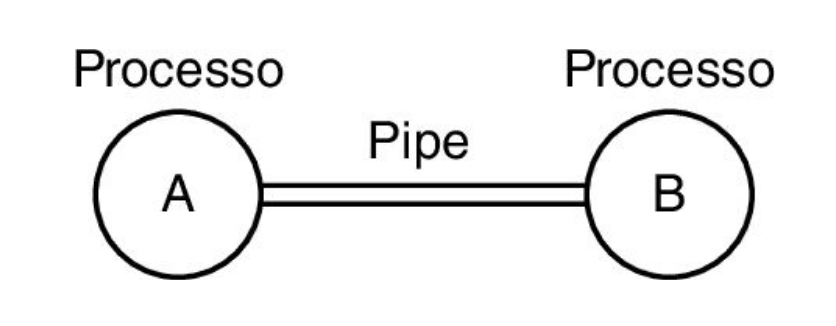
\includegraphics[width=0.4\linewidth]{Images/Screenshot 2024-12-18 at 13-24-07 so-01-intro-os.pptx - so-01-intro-os.pdf.png}
    \label{fig:enter-label}
\end{figure}

\paragraph{Pipe in Bash:} Le abbiamo viste con Ghini.
\textit{Esempio: A $||$ B}

\paragraph{Pipe in C:} Utilizza la funzione pipe() e i descrittori di file, permette la comunicazione tra processi correlati (es. genitore-figlio). Sono unidirezionali (ma possono essere create multiple pipe per bidirezionalità)
La creazione è esplicita nel codice del programma e persiste finché non viene chiusa o il processo termina.
\textit{Esempio:
pipe(pipefd)
… write(pipefd[1], ...)
… read(pipefd[0], …)}
